\documentclass{article}
\usepackage[utf8]{inputenc}
\usepackage{amsmath}
\usepackage{amssymb}
\usepackage{graphicx}

\begin{document}

\section*{Rank-one perturbations}
We are given the following pseudocode 
\begin{figure}[!hbt]
    \centering
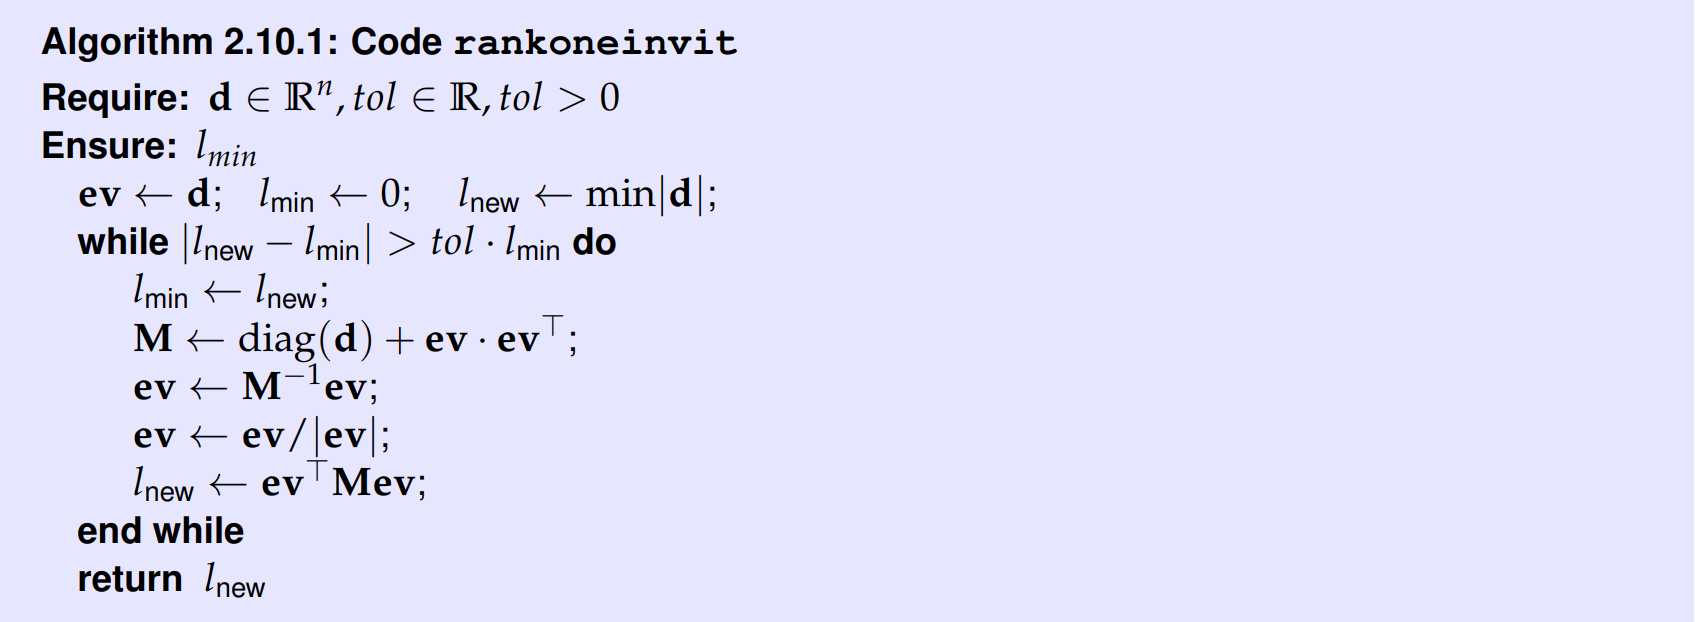
\includegraphics[width=1.0\linewidth]{PseudoCode2-10.png}
\end{figure}
Here \verb|diag| signifies a mapping that converts a vector into a diagonal matrix with the vector components as diagonal entries. A direct translation could look like the following code segment.
\begin{figure}[!hbt]
    \centering
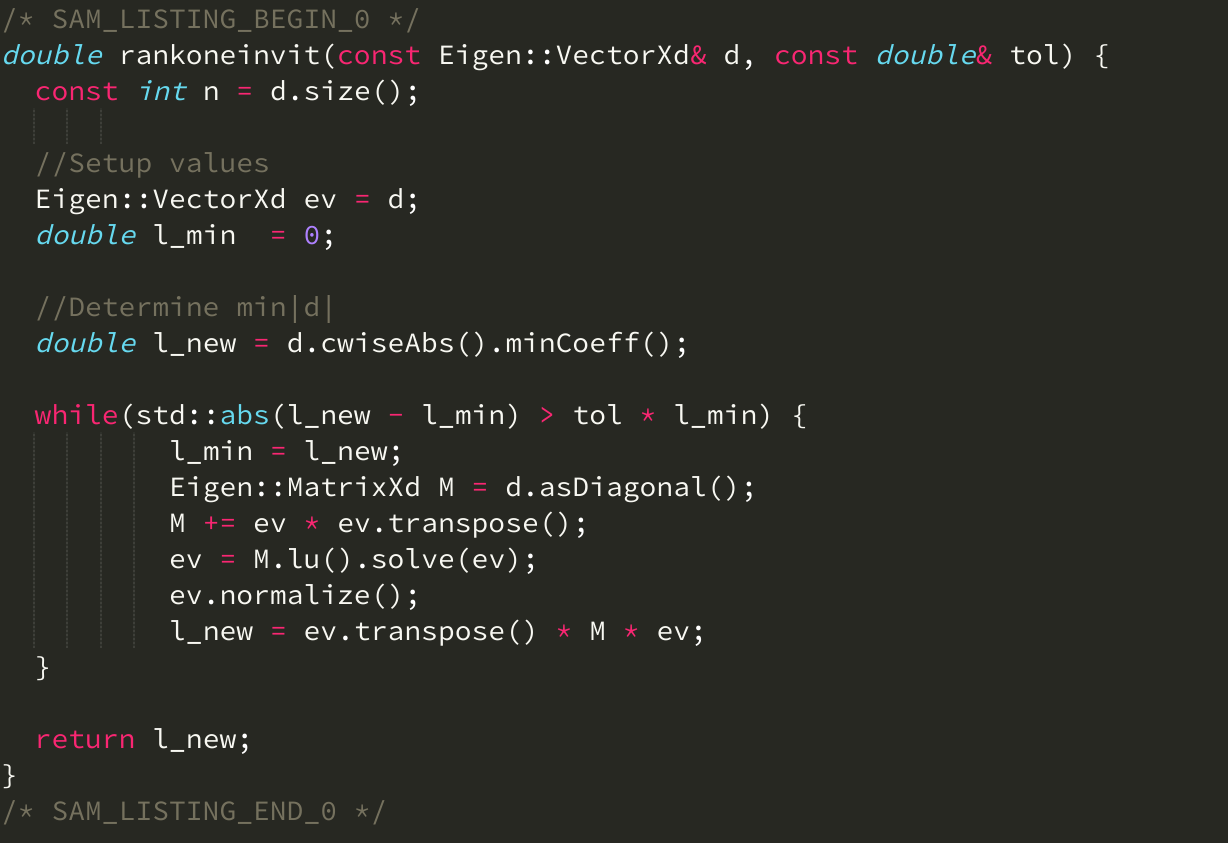
\includegraphics[width=1.0\linewidth]{2-10.a.png}
\end{figure}
The step \verb|M.lu().solve(ev)| is done because we have for some placeholder variable $\mathbf{x}$
\begin{equation*}
    \mathbf{M}\mathbf{x} = \mathbf{ev} \implies \mathbf{x} = \mathbf{M}^{-1}\mathbf{ev}
\end{equation*}
\subsection*{2-10.b}
We are tasked with stating the asymptotic complexity of the body of the loop in the function. Computing the matrix \verb|M| is done using matrix addition and an outer product which both can be done in $\mathcal{O}\left(n^{2}\right)$, the solving of a LSE can be done in $\mathcal{O}\left(n^{3}\right)$, normalizing is done in $\mathcal{O}\left(n\right)$ and the last product takes $\mathcal{O}\left(n^{2}\right)$. Hence overall we get $\mathcal{O}\left(n^{3}\right)$.

\subsection*{2-10.c}
The trick here is to use that we are doing a low rank modification to the diagonal matrix $D := \text{diag}\left(d_{1}, \dots, d_{n}\right)$. For $D$ we can compute $D^{-1}$ efficiently as we have
\begin{equation*}
    D^{-1}= \text{diag}\left(d_{1}, \dots, d_{n}\right)^{-1} =  \text{diag}\left(d_{1}^{-1}, \dots, d_{n}^{-1}\right)
\end{equation*}
we then use the Sherman-Morrison-Woodbury formula for the case $k=1$ and get
\begin{equation*}
    \mathbf{x} = \mathbf{A}^{-1}\mathbf{b} - \frac{\mathbf{A}^{-1}\mathbf{u}\left(\mathbf{v}^{\mathsf{H}}\left( \mathbf{A}^{-1}\mathbf{b}\right)\right)}{1 + \mathbf{v}^{\mathsf{H}}\left(\mathbf{A}^{-1}\mathbf{u}\right)}
\end{equation*}
We have in the code segment that $M = D + ev \cdot ev^{\mathsf{T}}$, hence we have $\mathbf{A} = \mathbf{D}$, $\mathbf{u} = \mathbf{ev}$, $\mathbf{v} = \mathbf{ev}$ and $\mathbf{x}$ is the new value for $\mathbf{ev}$ after normalizing it in the equation, which then gives us the following equation.
\begin{equation*}
    \mathbf{x} = \mathbf{D}^{-1}\mathbf{b} - \frac{\mathbf{D}^{-1}\mathbf{ev}\left(\mathbf{ev}^{\mathsf{H}}\left( \mathbf{D}^{-1}\mathbf{b}\right)\right)}{1 + \mathbf{ev}^{\mathsf{H}}\left(\mathbf{D}^{-1}\mathbf{ev}\right)}
\end{equation*}
We want to solve the equation $\mathbf{D}\mathbf{x} = \mathbf{ev}$, hence we also have $\mathbf{b} = \mathbf{ev}$, which leads to the final equation (here $\mathbf{x}$ is the new value of $\mathbf{ev}$)
\begin{align*}
    \mathbf{x} &= \mathbf{D}^{-1}\mathbf{ev} - \frac{\mathbf{D}^{-1}\mathbf{ev}\left(\mathbf{ev}^{\mathsf{H}}\left( \mathbf{D}^{-1}\mathbf{ev}\right)\right)}{1 + \mathbf{ev}^{\mathsf{H}}\left(\mathbf{D}^{-1}\mathbf{ev}\right)} \\
    &=\frac{\mathbf{D}^{-1}\mathbf{ev}\left(1 + \mathbf{ev}^{\mathsf{H}}\left(\mathbf{D}^{-1}\mathbf{ev}\right)\right)}{1 + \mathbf{ev}^{\mathsf{H}}\left(\mathbf{D}^{-1}\mathbf{ev}\right)} - \frac{\mathbf{D}^{-1}\mathbf{ev}\left(\mathbf{ev}^{\mathsf{H}}\left( \mathbf{D}^{-1}\mathbf{ev}\right)\right)}{1 + \mathbf{ev}^{\mathsf{H}}\left(\mathbf{D}^{-1}\mathbf{ev}\right)} \\
    &=\frac{\mathbf{D}^{-1}\mathbf{ev}+ \mathbf{D}^{-1}\mathbf{ev}\left(\mathbf{ev}^{\mathsf{H}}\left(\mathbf{D}^{-1}\mathbf{ev}\right)\right)}{1 + \mathbf{ev}^{\mathsf{H}}\left(\mathbf{D}^{-1}\mathbf{ev}\right)} - \frac{\mathbf{D}^{-1}\mathbf{ev}\left(\mathbf{ev}^{\mathsf{H}}\left( \mathbf{D}^{-1}\mathbf{ev}\right)\right)}{1 + \mathbf{ev}^{\mathsf{H}}\left(\mathbf{D}^{-1}\mathbf{ev}\right)} \\
    &= \frac{\mathbf{D}^{-1}\mathbf{ev}}{1 + \mathbf{ev}^{\mathsf{H}}\left(\mathbf{D}^{-1}\mathbf{ev}\right)} \\
    &= \mathbf{D}^{-1}\mathbf{ev}\cdot \frac{1}{1 + \mathbf{ev}^{\mathsf{H}}\left(\mathbf{D}^{-1}\mathbf{ev}\right)}
\end{align*}

\pagebreak

\noindent We hence compute $\mathbf{D^{-1}}$ by taking the inverse of the diagonal elements $d_{ii}^{-1}$ and then use the equation above to get the the new value for $\mathbf{ev}$. We must be careful now, as we are still computing inefficient outer products, which we must avoid. The product $\mathbf{D}^{-1}\mathbf{ev}$ is a matrix-vector product with a diagonal matrix and can thus just be made using \verb|cwiseProduct|. The other outer product $\mathbf{ev}^{\mathsf{T}}\mathbf{M}\mathbf{ev}$ is a bit more complicated and requires a bit more thought. We compute $\mathbf{M} = \mathbf{D} + \mathbf{ev} \cdot \mathbf{ev}^{\mathsf{T}}$. We hence have overall (where we denote by $\mathbf{ev}_{\text{old}}$ the old value of $\mathbf{ev}$.)
\begin{align*}
    \mathbf{ev}^{\mathsf{T}} \mathbf{M}\mathbf{ev} = \mathbf{ev}^{\mathsf{T}}\left(\mathbf{D} + \mathbf{ev}_{\text{old}} \cdot \mathbf{ev}_{\text{old}}^{\mathsf{T}}\right)\mathbf{ev} &= \left(\mathbf{ev}^{\mathsf{T}}\mathbf{D} + \mathbf{ev}^{\mathsf{T}}\mathbf{ev}_{\text{old}}\mathbf{ev}_{\text{old}}^{\mathsf{T}}\right)\mathbf{ev} \\
    &=\mathbf{ev}^{\mathsf{T}}\mathbf{D}\mathbf{ev} + \mathbf{ev}^{\mathsf{T}}\mathbf{ev}_{\text{old}}\mathbf{ev}_{\text{old}}^{\mathsf{T}}\mathbf{ev} \\
    &=\mathbf{ev}^{\mathsf{T}}\mathbf{D}\mathbf{ev} + \left(\mathbf{ev}^{\mathsf{T}}\mathbf{ev}_{\text{old}}\right)^{2} \quad \text{($ \mathbf{ev}_{\text{old}}^{\mathsf{T}}\mathbf{ev} = \mathbf{ev}^{\mathsf{T}}\mathbf{ev}_{\text{old}}$)}
\end{align*}
The term $\mathbf{ev}_{\text{old}}$ comes from us decomposing $\mathbf{M}$ into $\mathbf{D} + \mathbf{ev}_{\text{old}} \cdot \mathbf{ev}_{\text{old}}^{\mathsf{T}}$ which is how we constructed the current $\mathbf{M}$ and hence we must distinguish between $\mathbf{ev}_{\text{old}}$ and $\mathbf{ev}$ as otherwise our implementation would not be correct.
Both of these products can fully be implemented using only \verb|cwiseProduct| and inner products, which both have $\mathcal{O}\left(n\right)$ as there asymptotic complexity.

\begin{figure}[!hbt]
    \centering
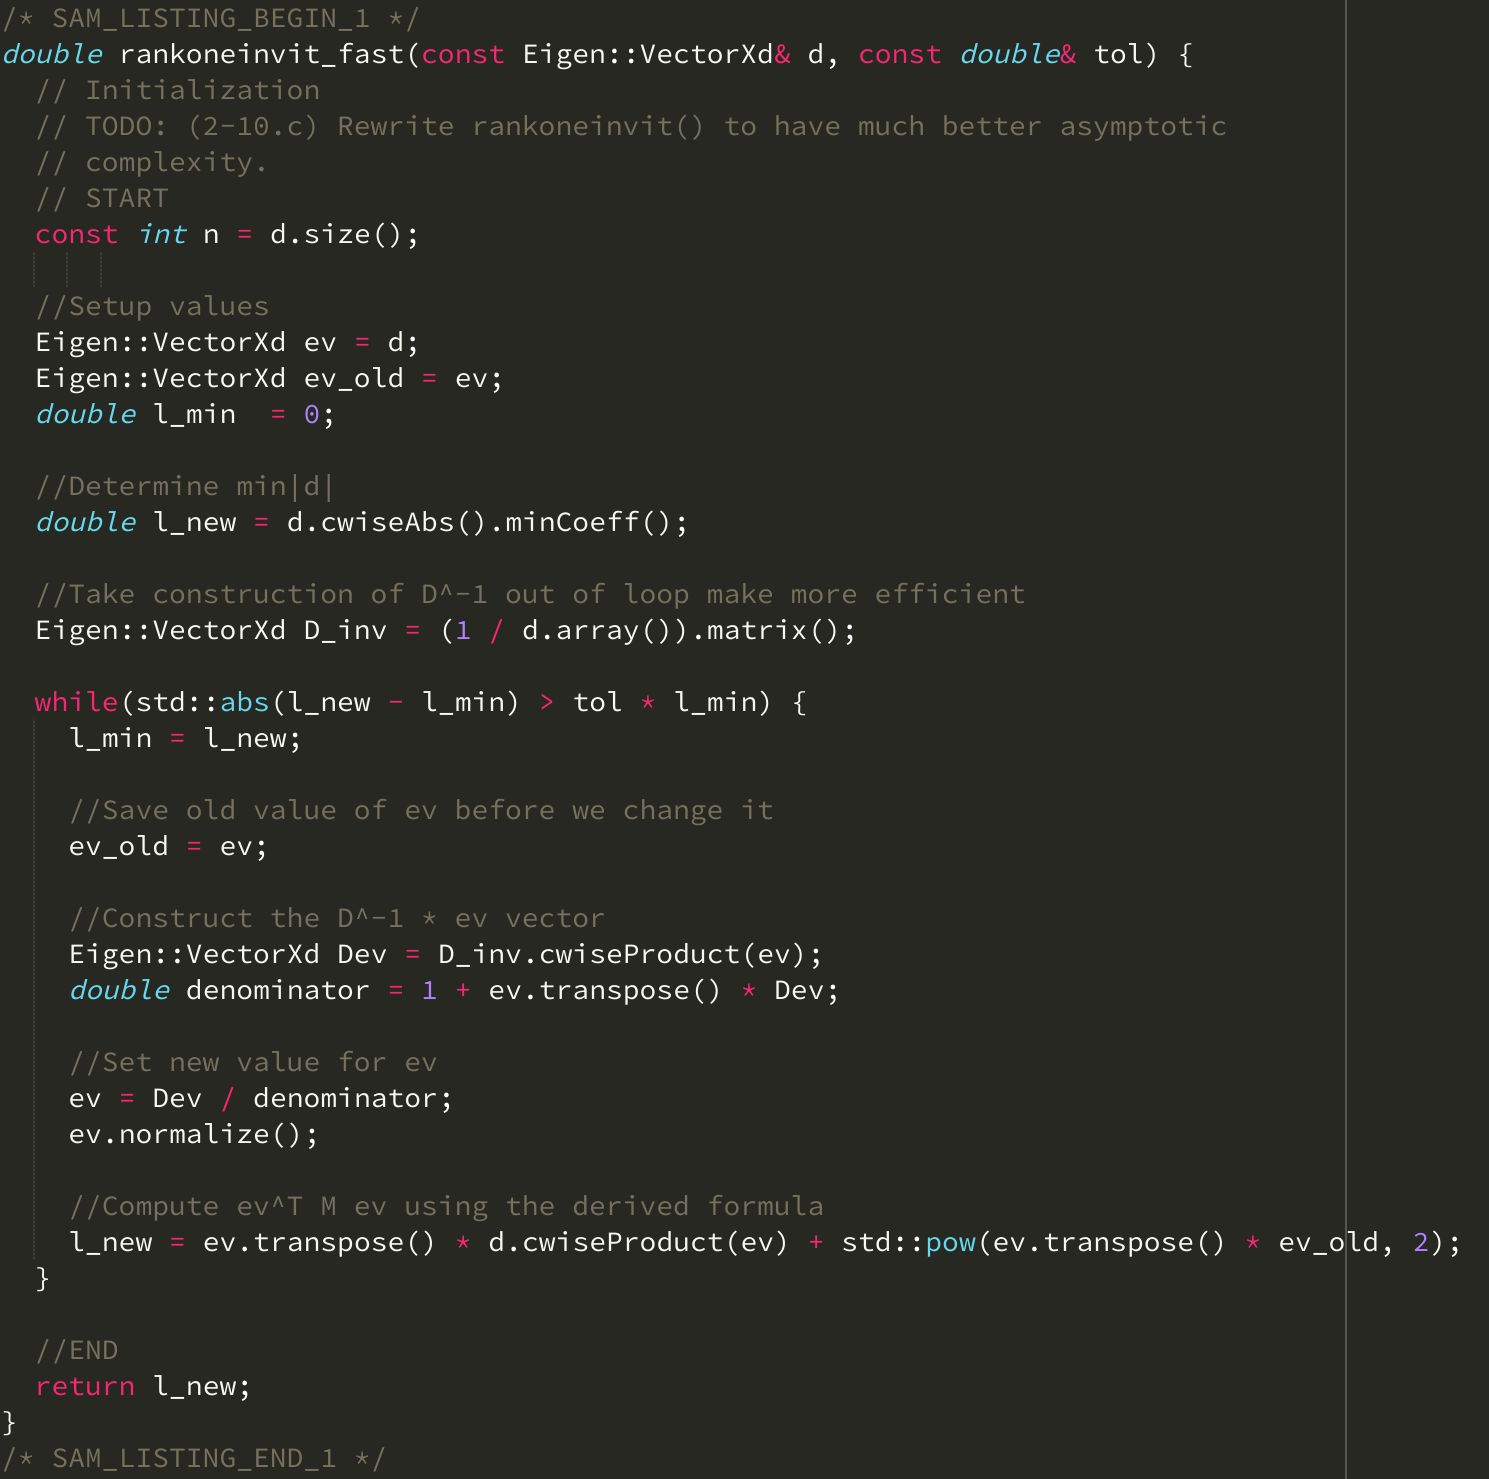
\includegraphics[width=0.9\linewidth]{2-10.c.png}
\end{figure}


\subsection*{2-10.d} 
We are tasked with giving the asymptotic complexity of the execution of the loop body in the efficient implementation. We know that all \verb|cwiseProduct| and inner products $\mathbf{x}^{\mathsf{T}}\mathbf{x}$ have an asymptotic runtime of $\mathcal{O}\left(n\right)$, all vectorized operations used also operate in $\mathcal{O}\left(n\right)$, hence we get an overall runtime of $\mathcal{O}\left(n\right)$.
\subsection*{2-10.e}
Given without reasoning.
\begin{figure}[!hbt]
    \centering
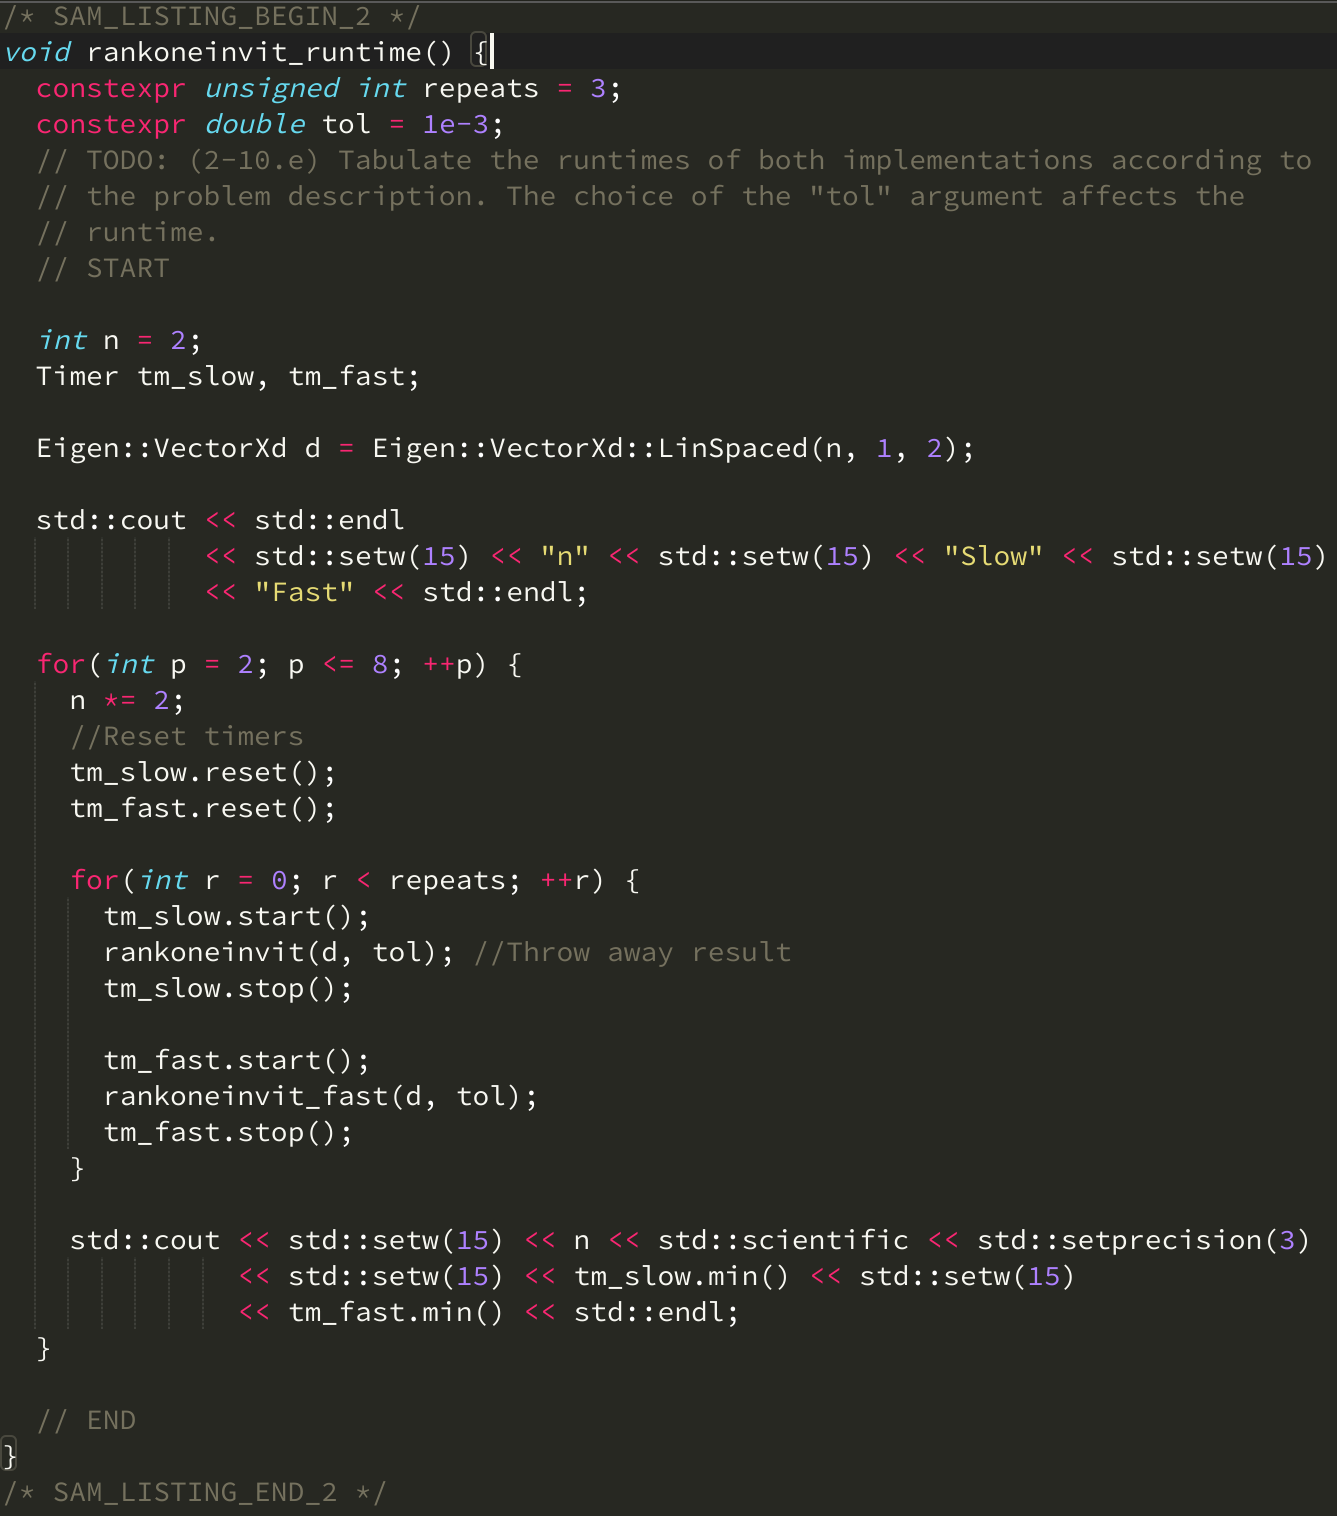
\includegraphics[width=1.0\linewidth]{2-10.e.png}
\end{figure}


\end{document}
